\chapter{Prezentacja aplikacji}
	W projekcie zaimplementowane zostąły podstawowe widoki wykorzystujące stworzoną architekturę.
\section{Rejestracja i logowanie}
	\begin{figure}[H]
		\centering
		\begin{minipage}{.5\textwidth}
			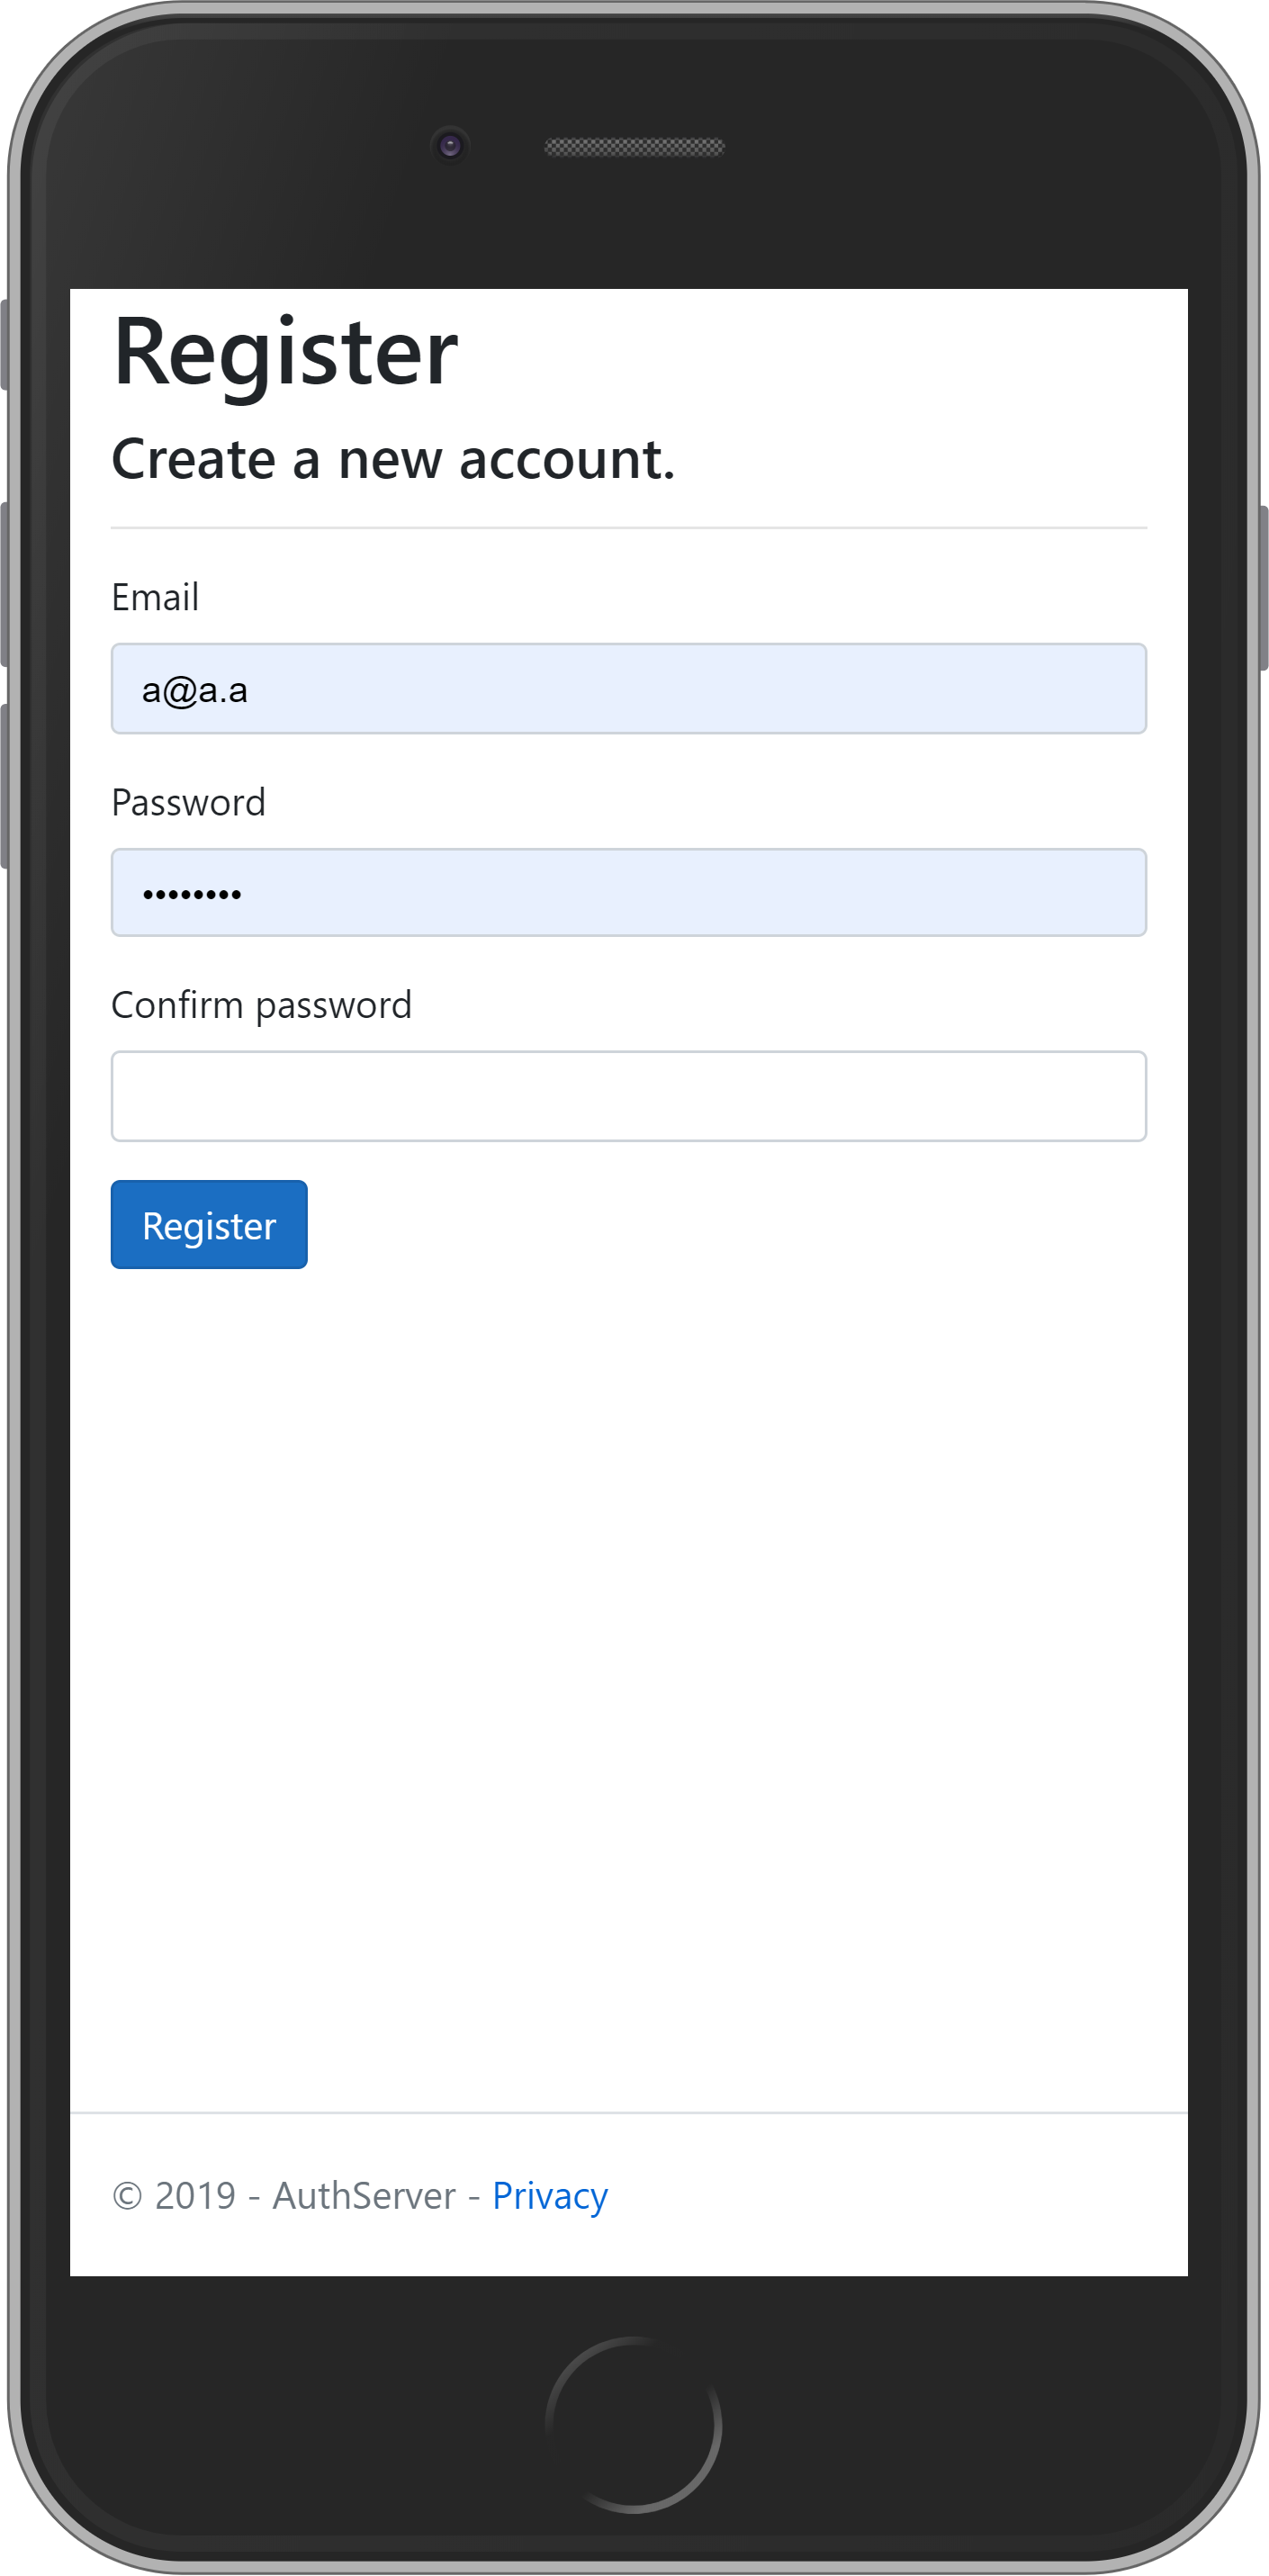
\includegraphics[width=0.9\linewidth]{rys06/register.png}
		\end{minipage}%
		\begin{minipage}{0.5\textwidth}
			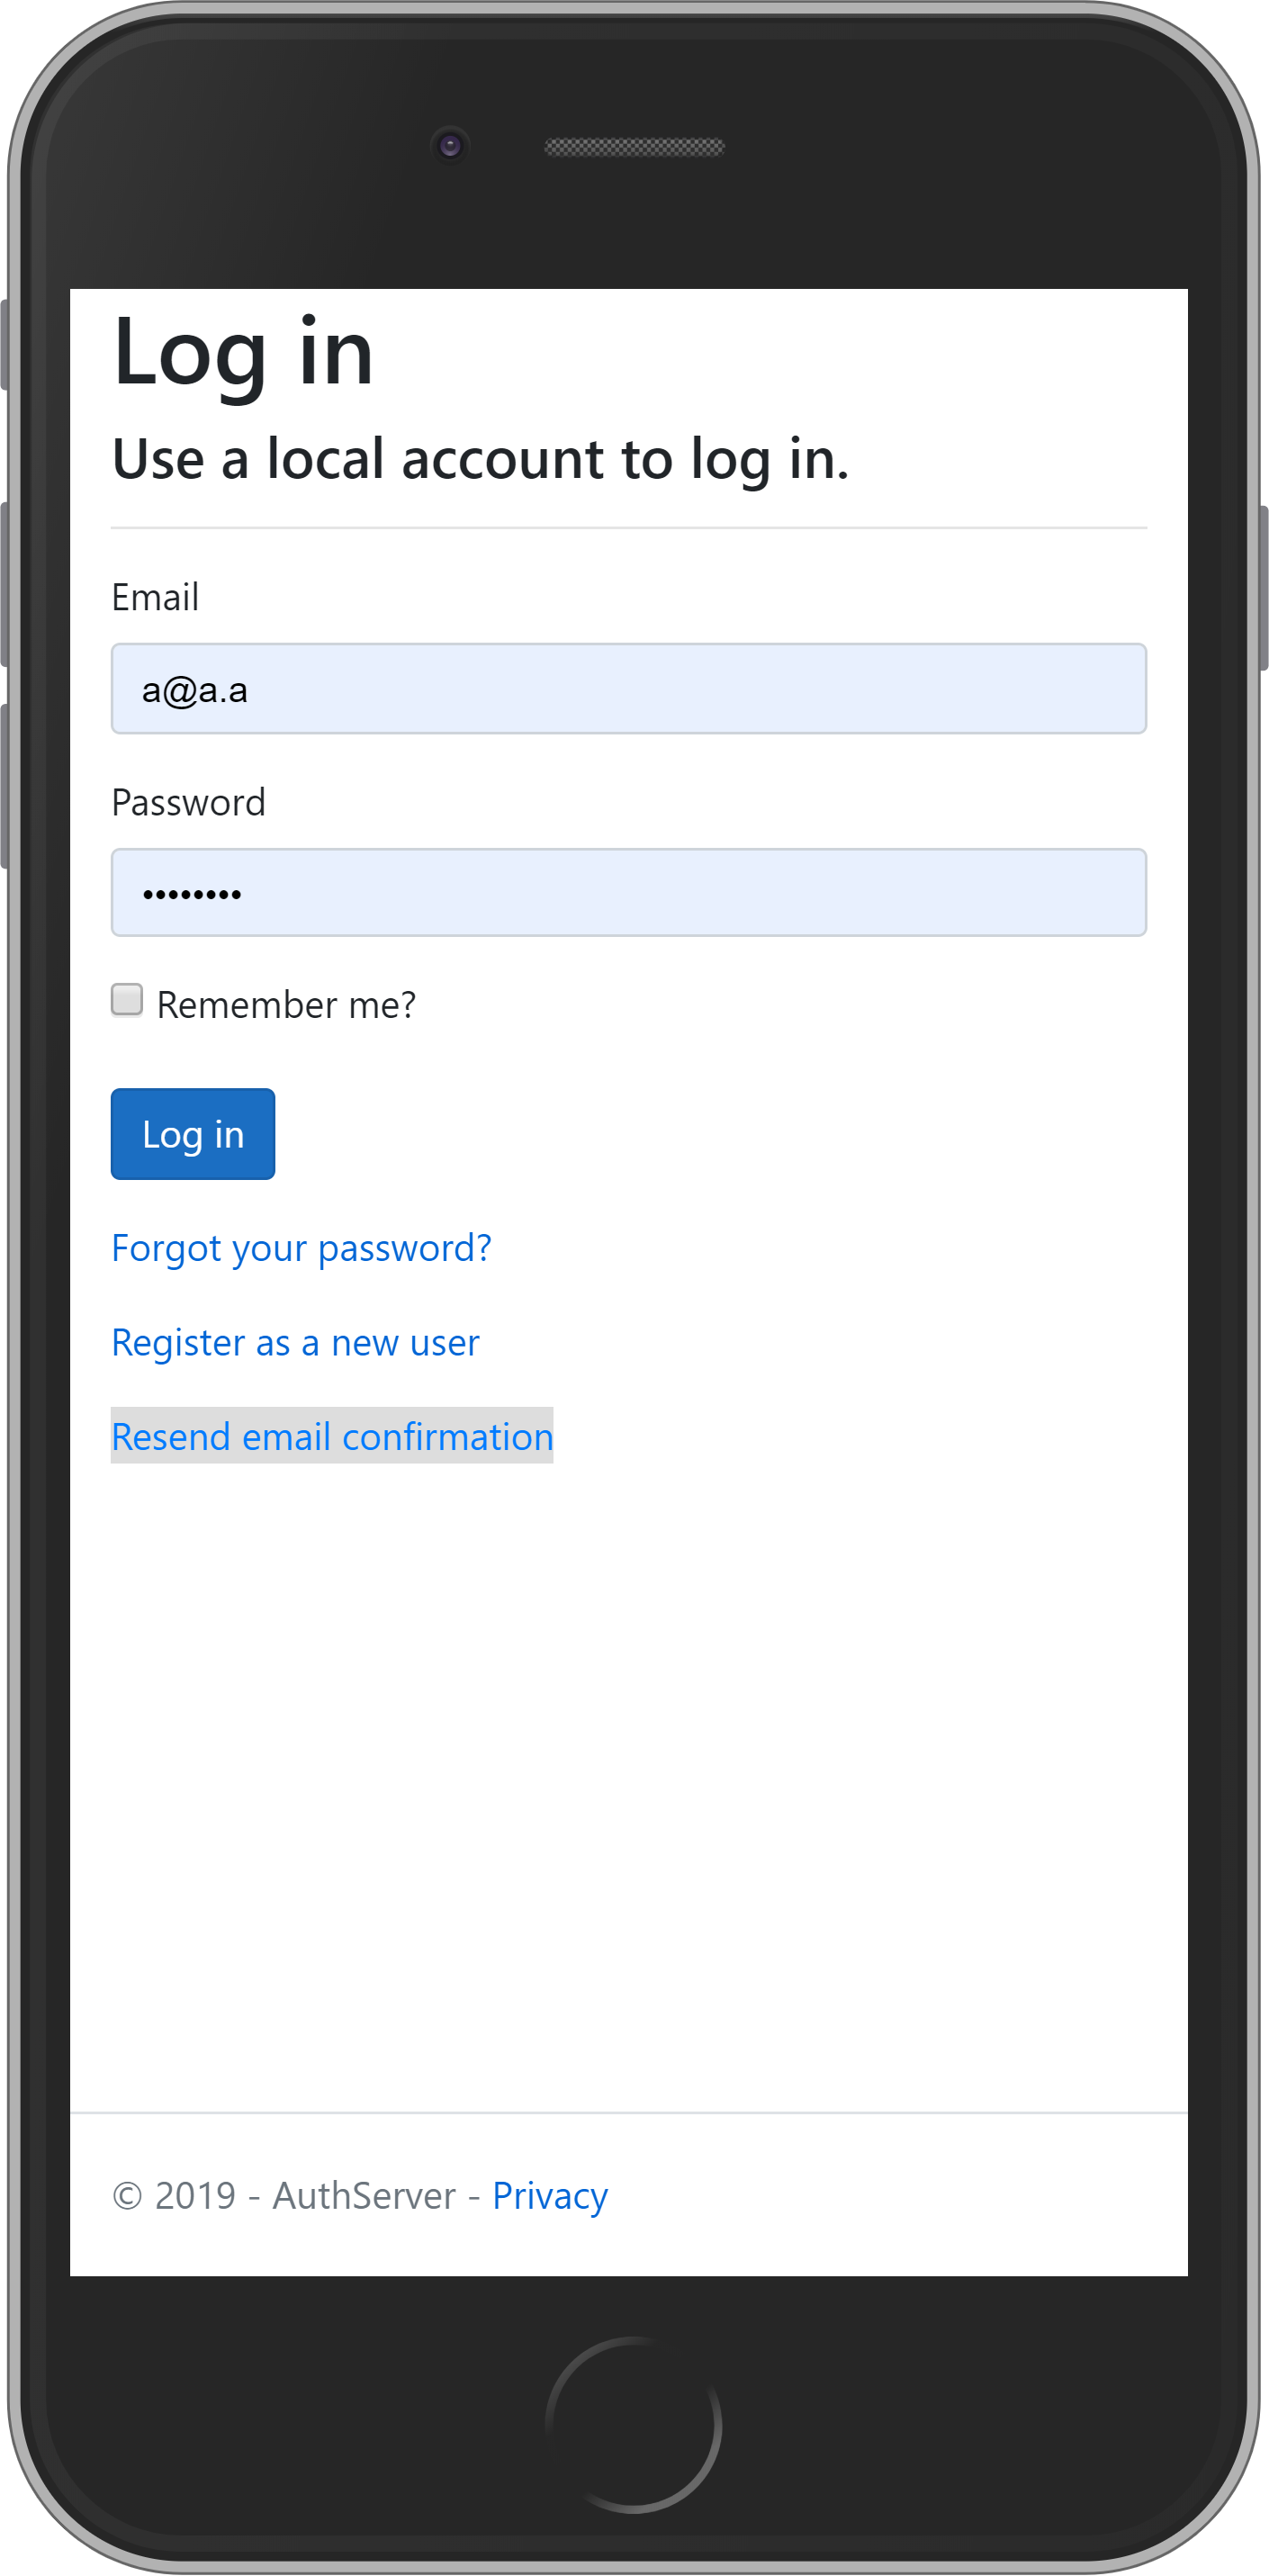
\includegraphics[width=0.9\linewidth]{rys06/login.png}
		\end{minipage}
		\caption{Ekrany rejestracji i logowania}
		\label{fig:login}
	\end{figure}

\section{Widoki albumów}
	\begin{figure}[H]
		\centering
		\begin{minipage}{.5\textwidth}
			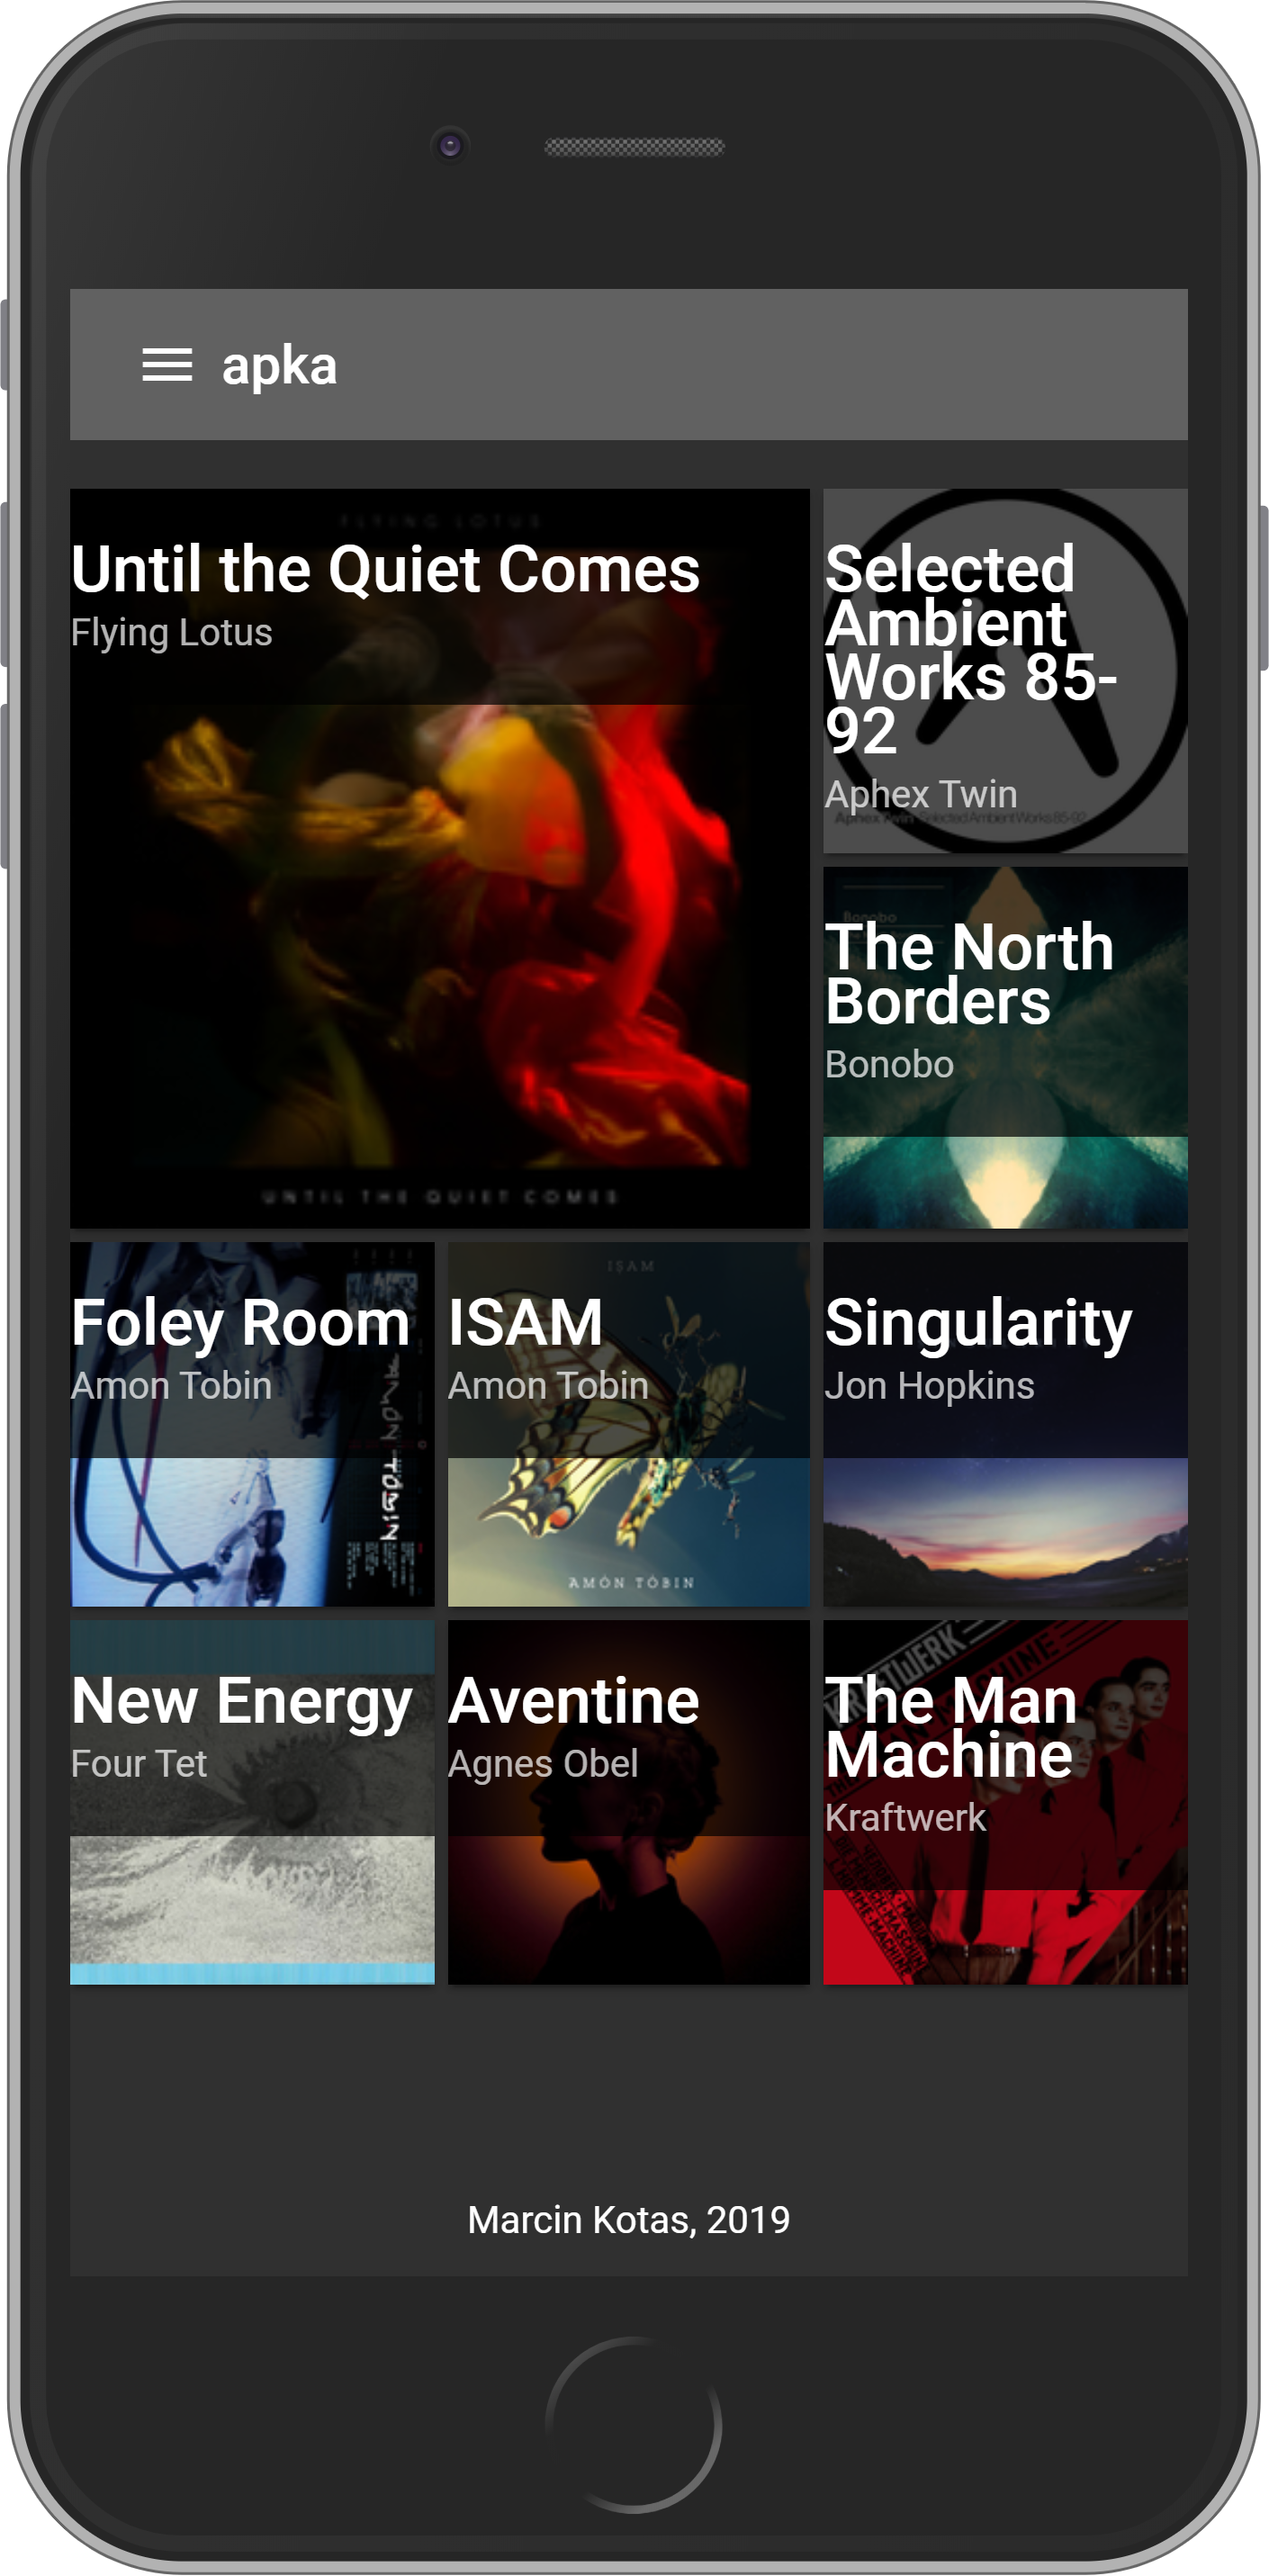
\includegraphics[width=0.9\linewidth]{rys06/explore.png}
		\end{minipage}%
		\begin{minipage}{0.5\textwidth}
			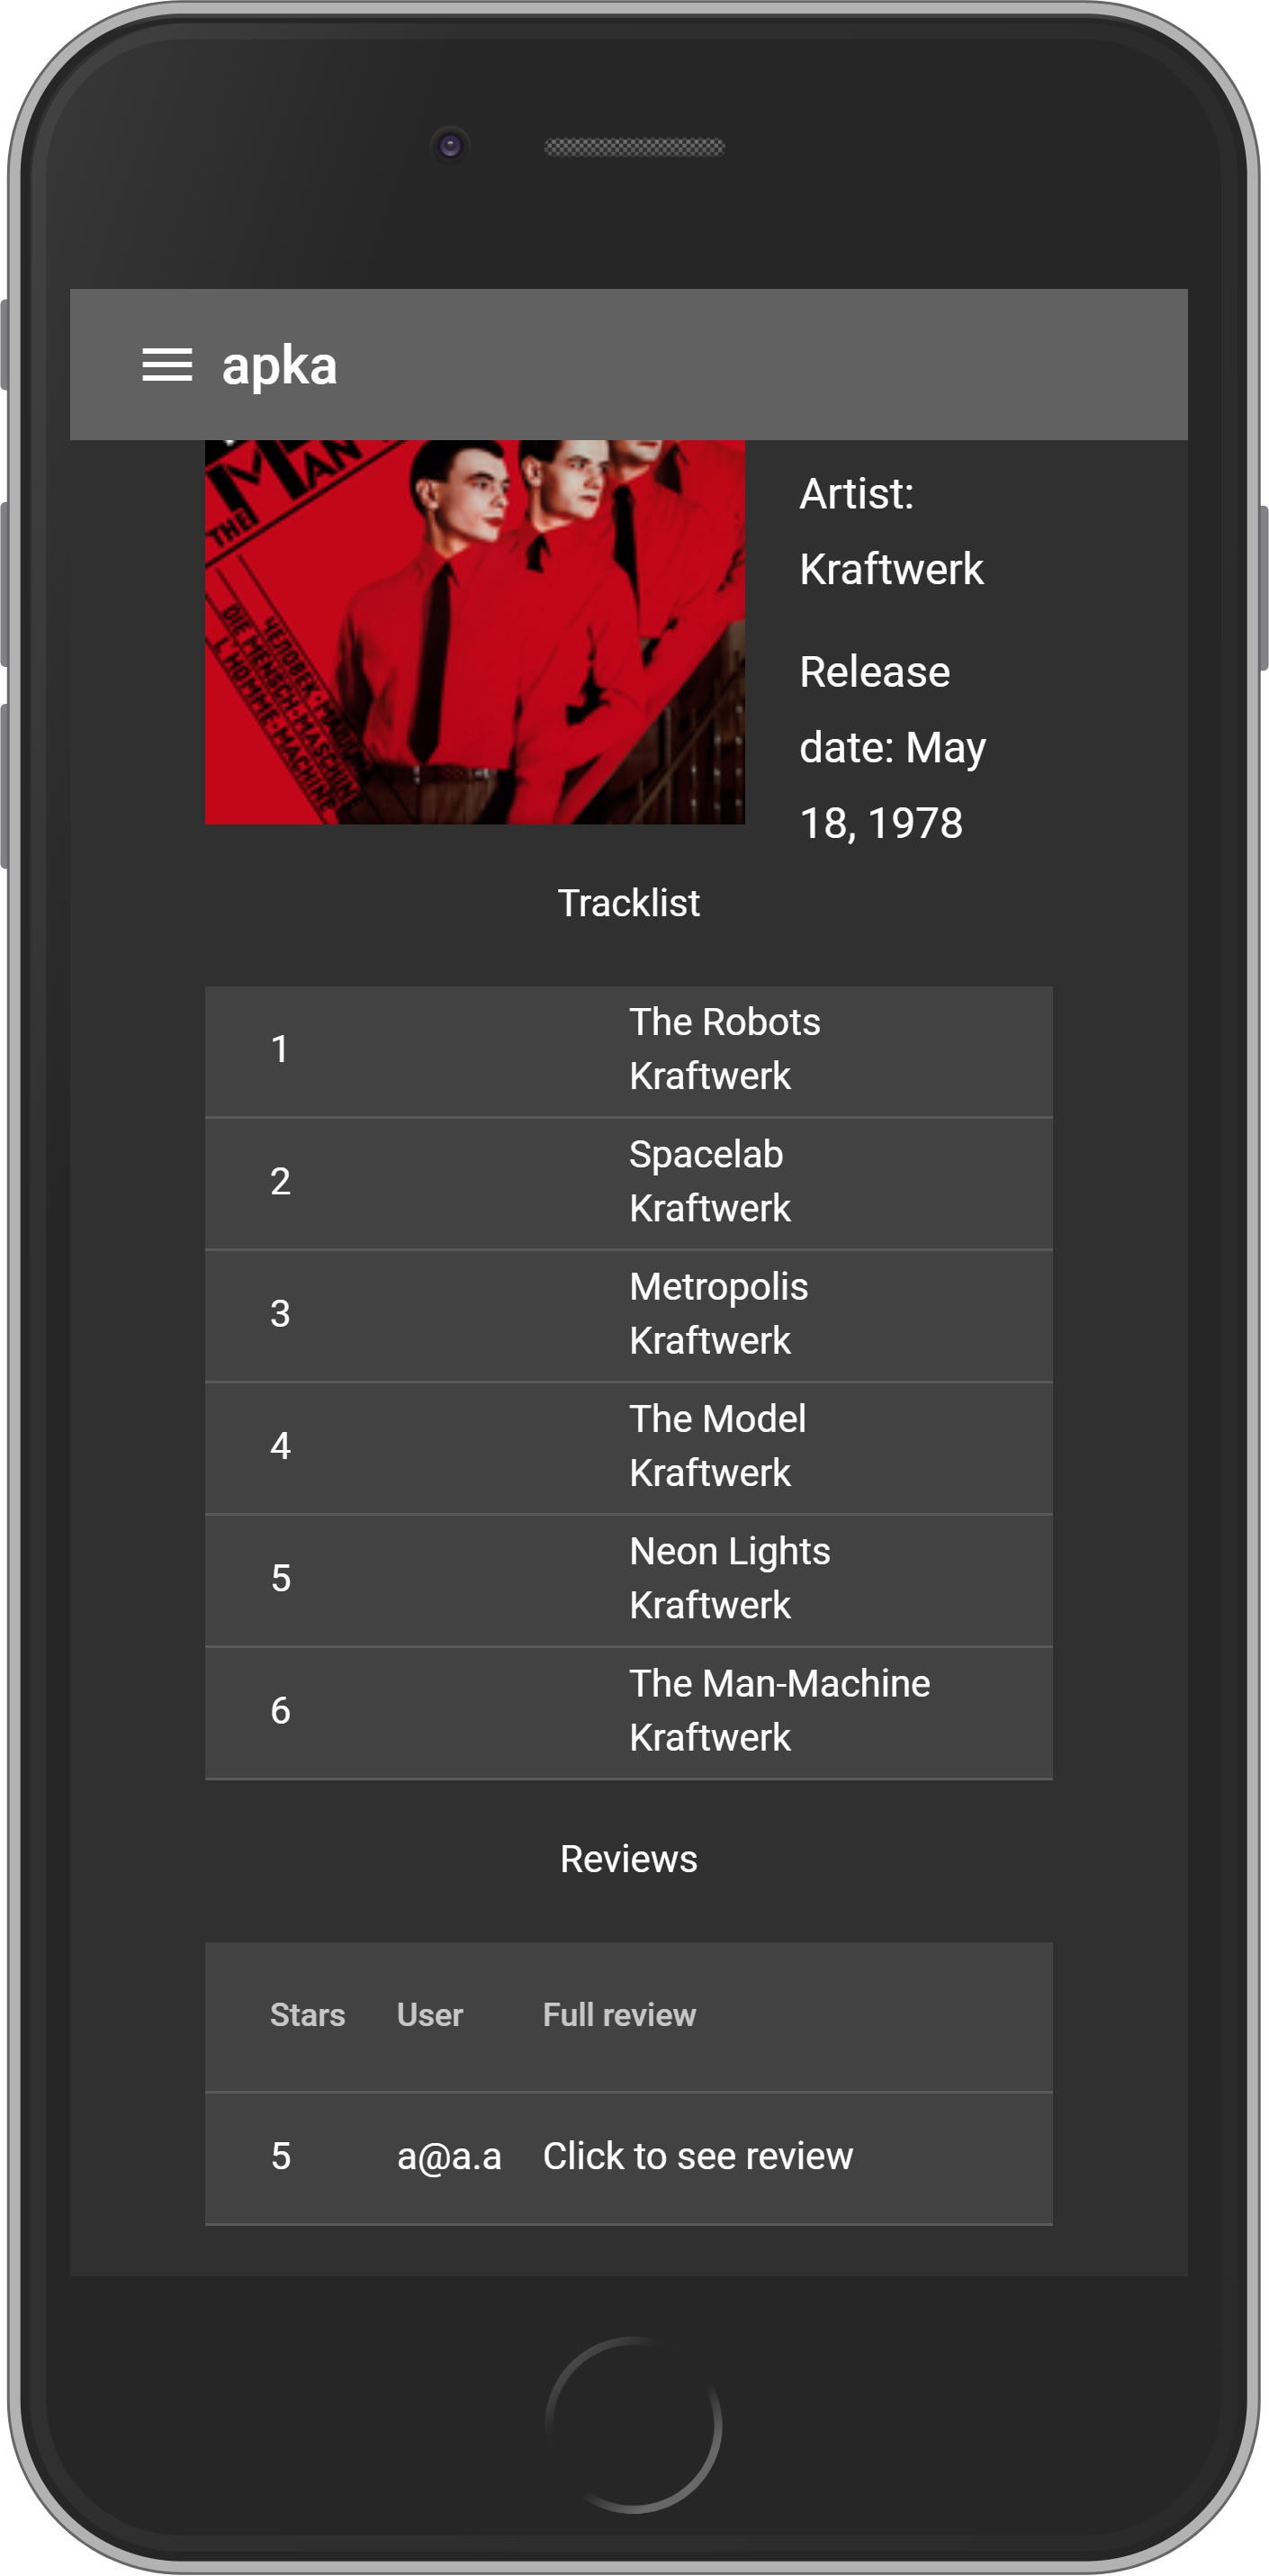
\includegraphics[width=0.9\linewidth]{rys06/album.png}
		\end{minipage}
		\caption{Ekrany wyświetlania listy albumów i szczegółów albumu}
		\label{fig:album}
	\end{figure}
	
\section{Dodawanie oceny}
	\begin{figure}[H]
		\centering
		\begin{minipage}{.5\textwidth}
			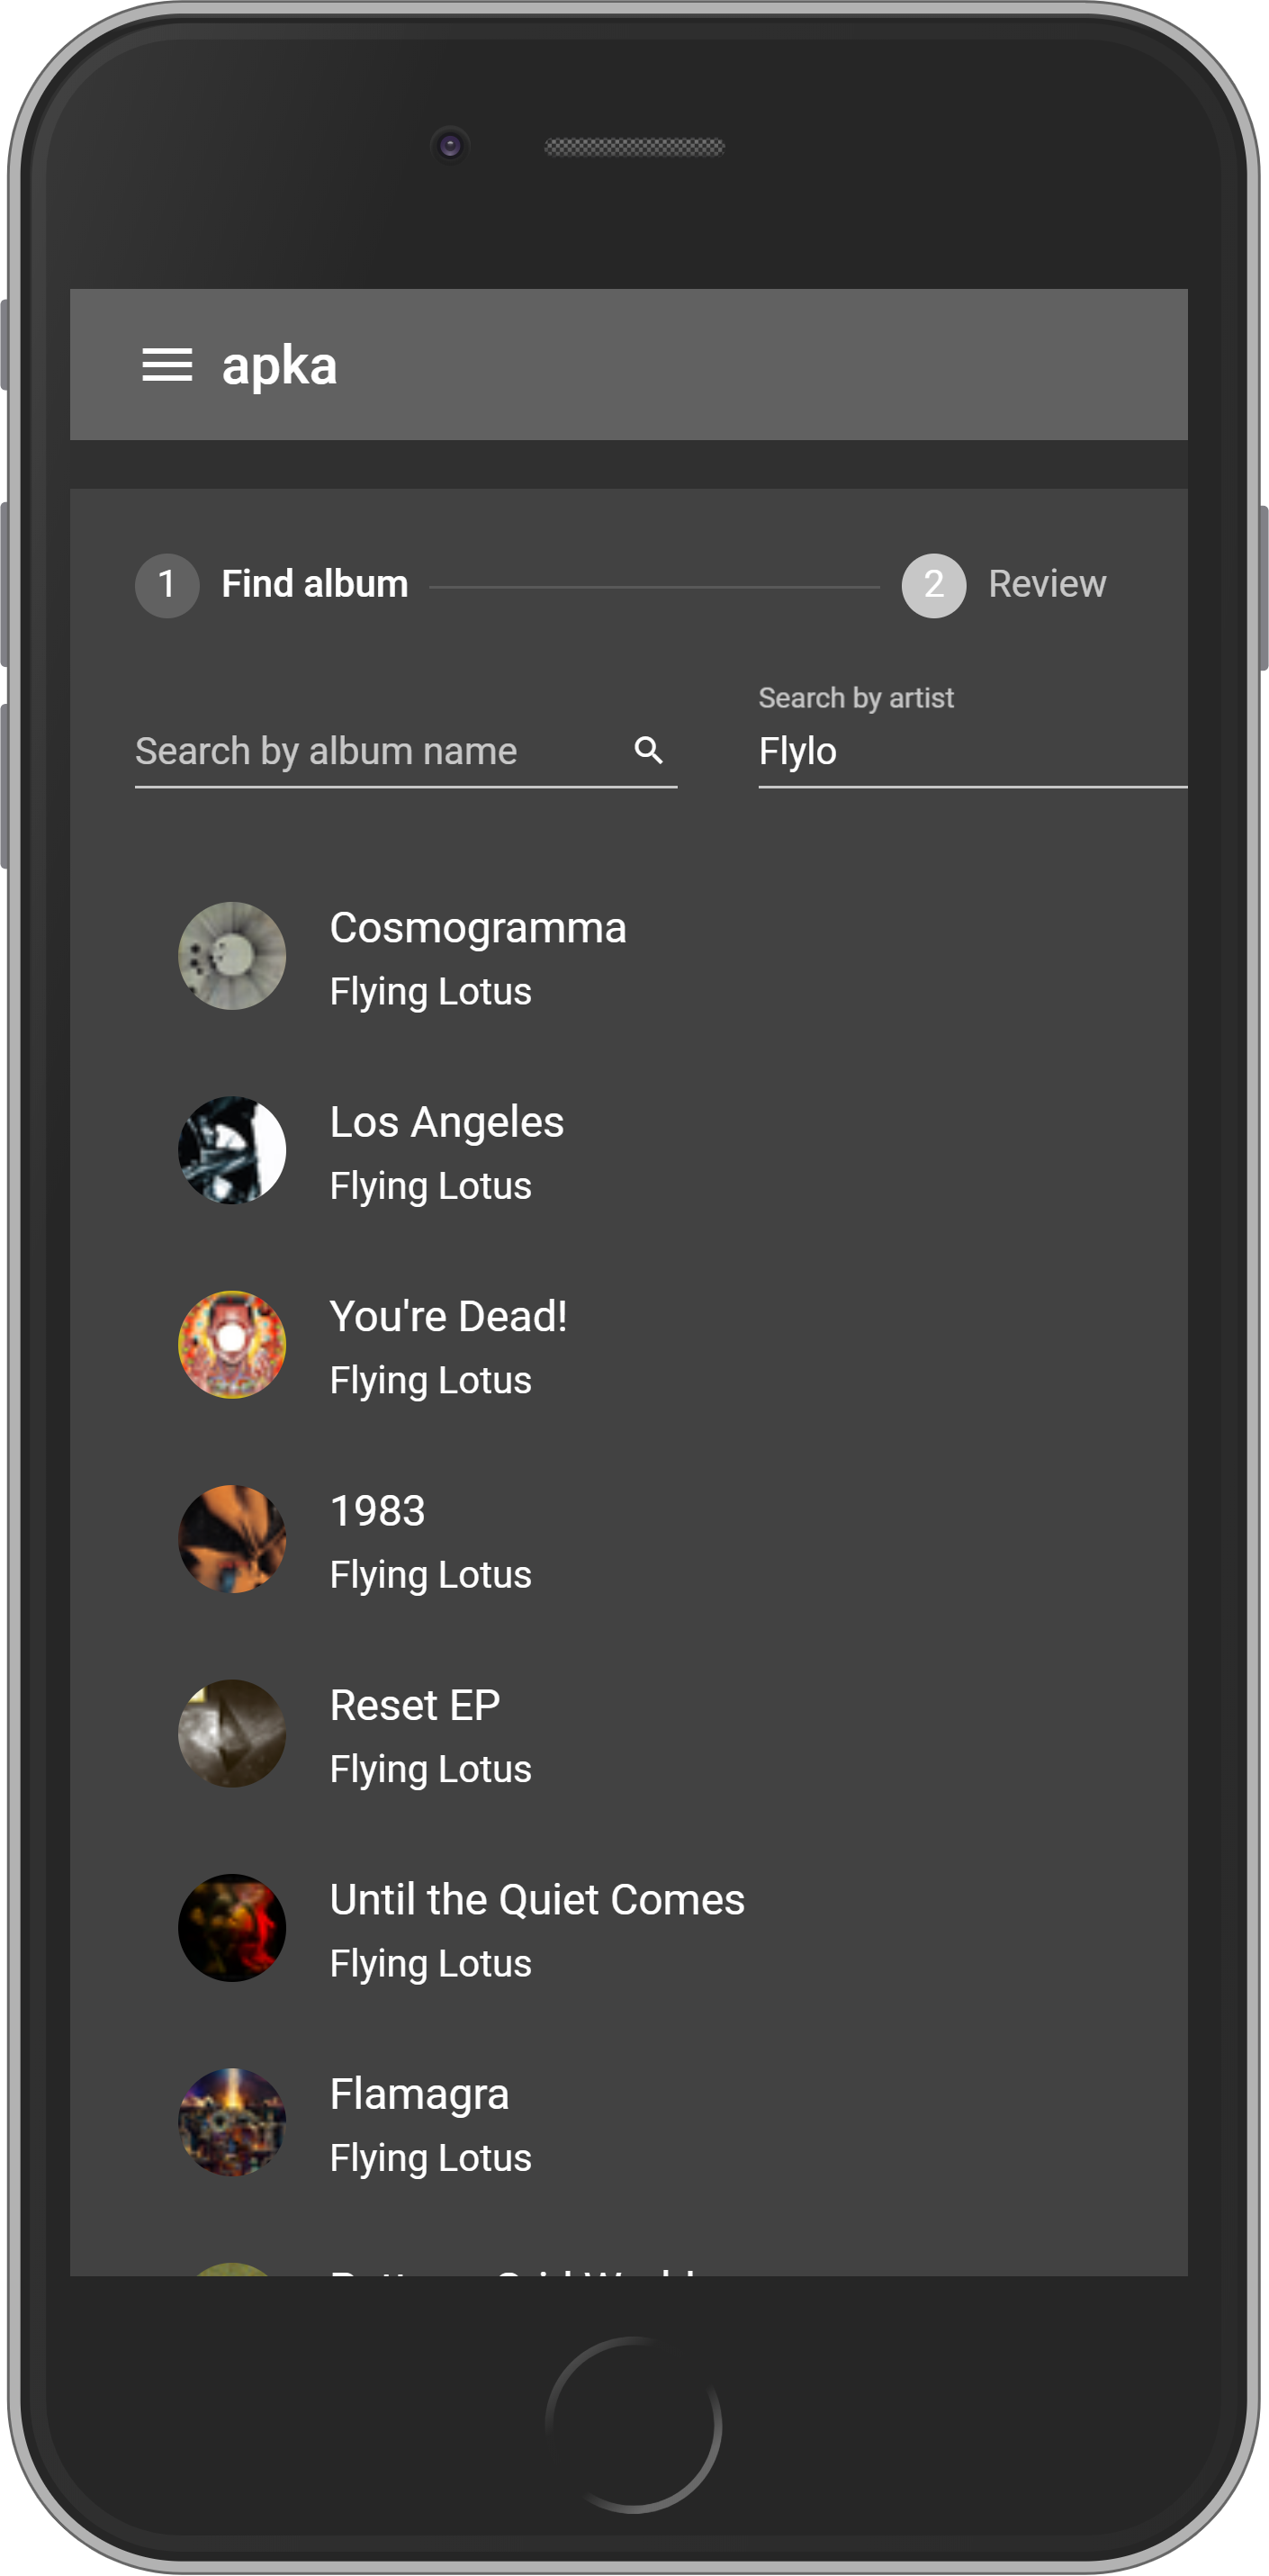
\includegraphics[width=0.9\linewidth]{rys06/search.png}
		\end{minipage}%
		\begin{minipage}{0.5\textwidth}
			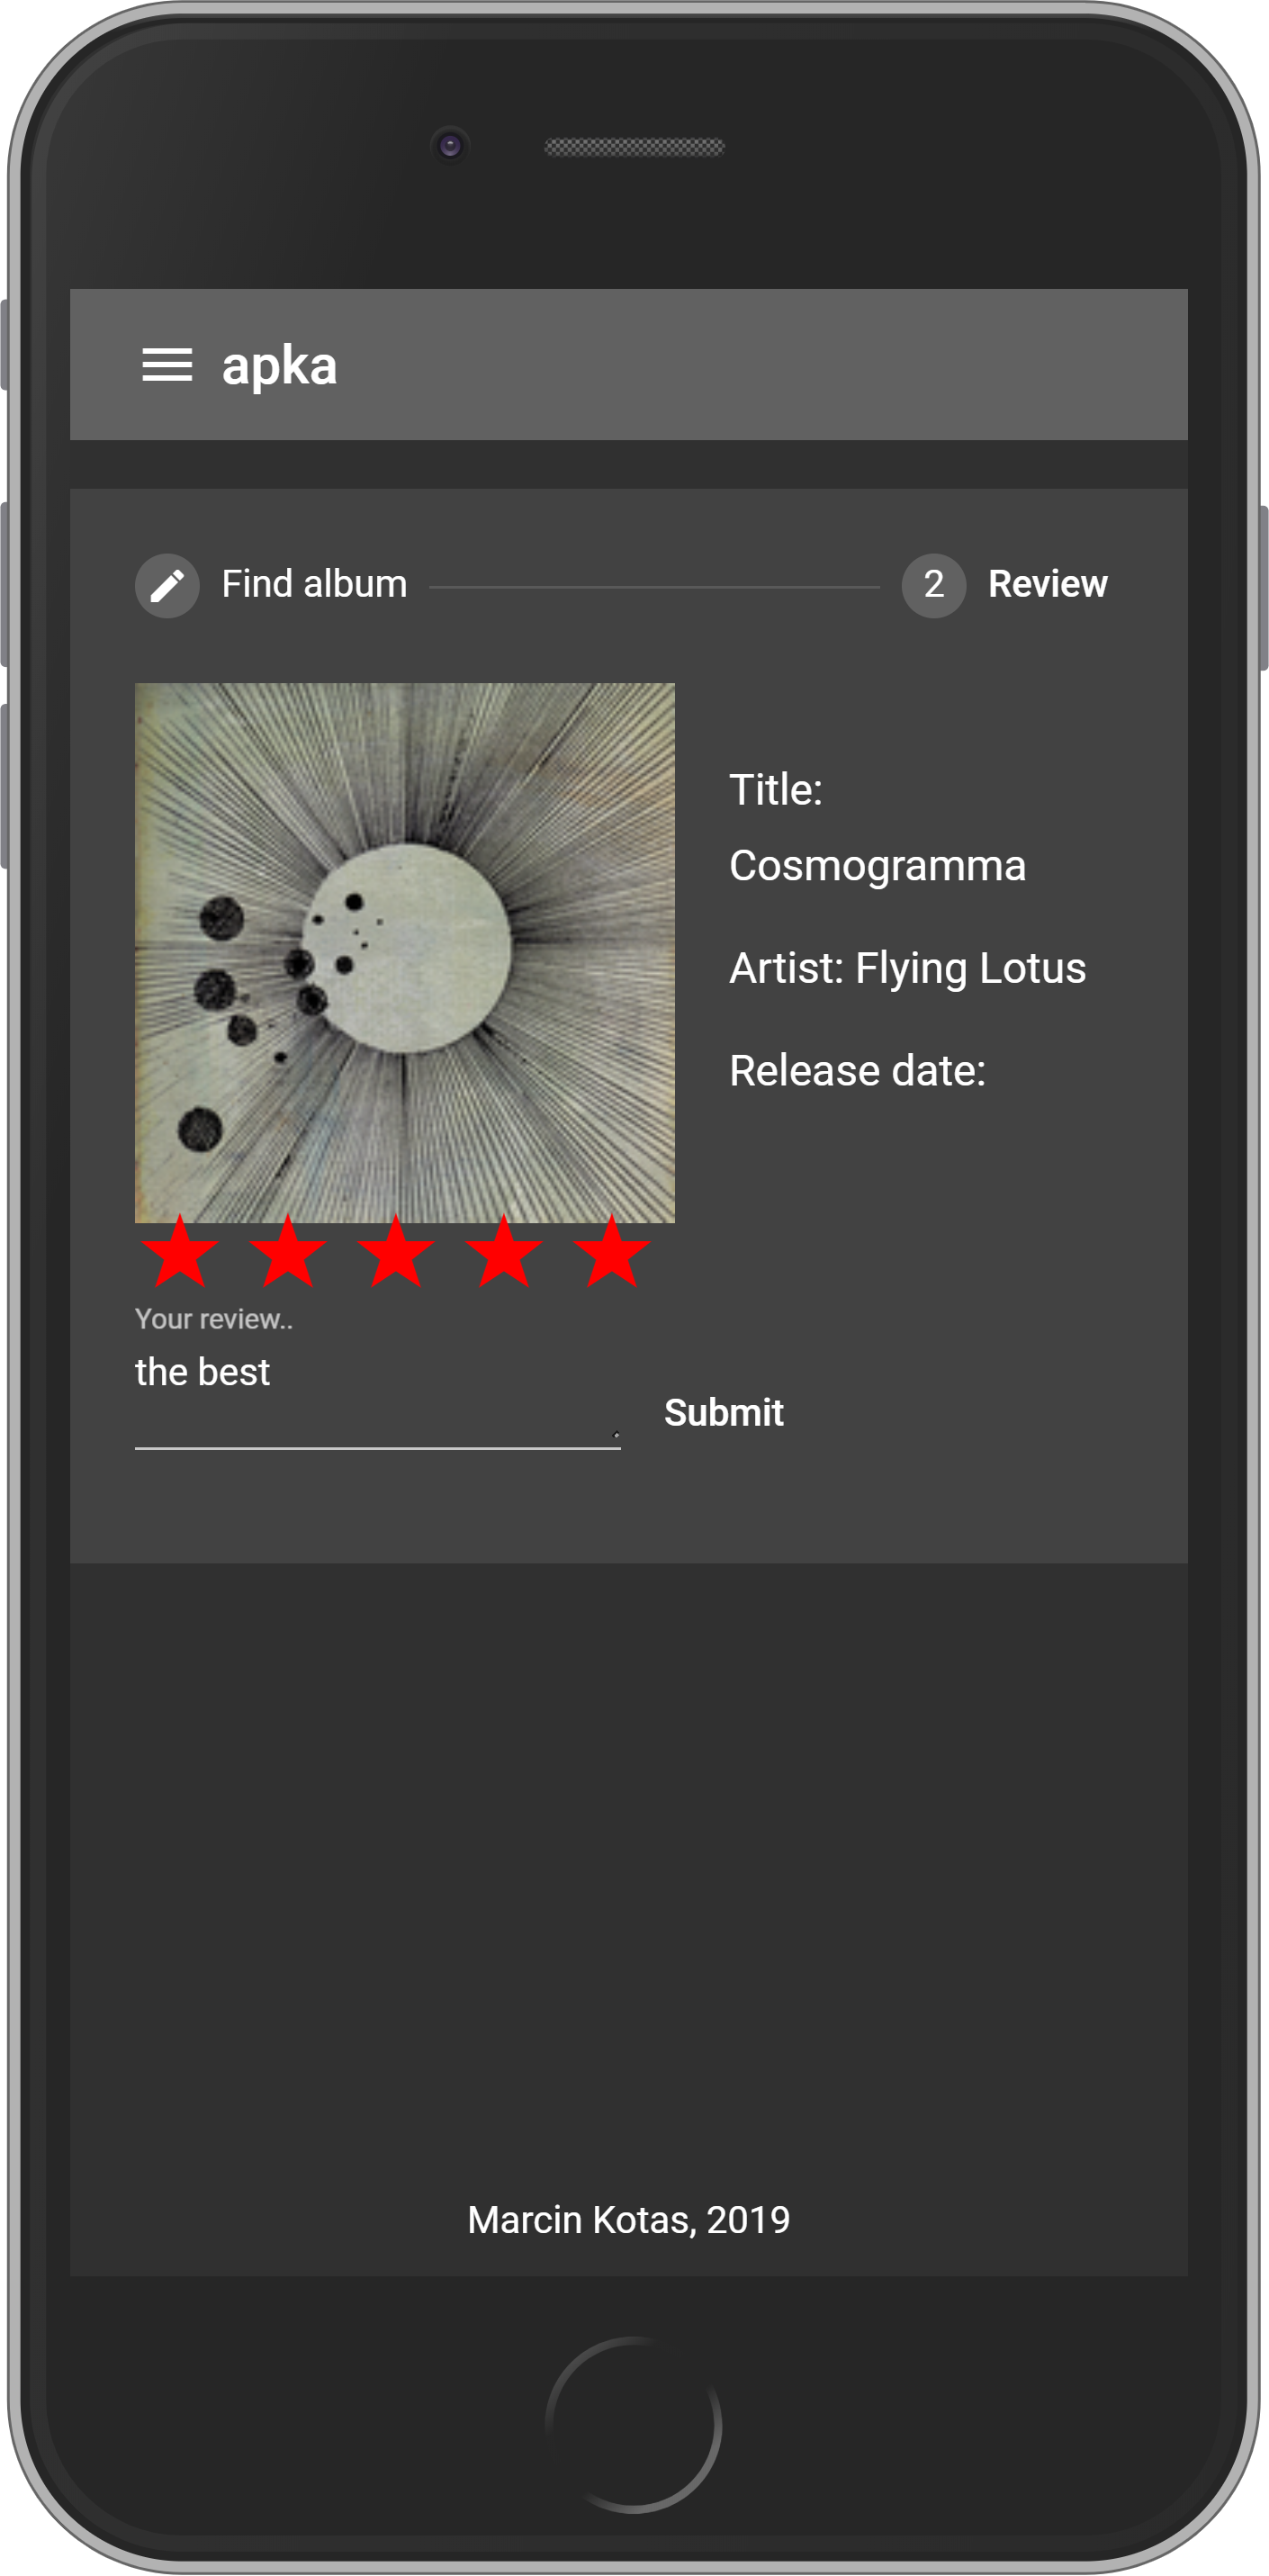
\includegraphics[width=0.9\linewidth]{rys06/rate.png}
		\end{minipage}
		\caption{Ekrany wyszukiwania albumu i dodawania oceny}
		\label{fig:rating}
	\end{figure}
	
\section{Jasny motyw}
	\begin{figure}[H]
		\centering
		\begin{minipage}{.5\textwidth}
			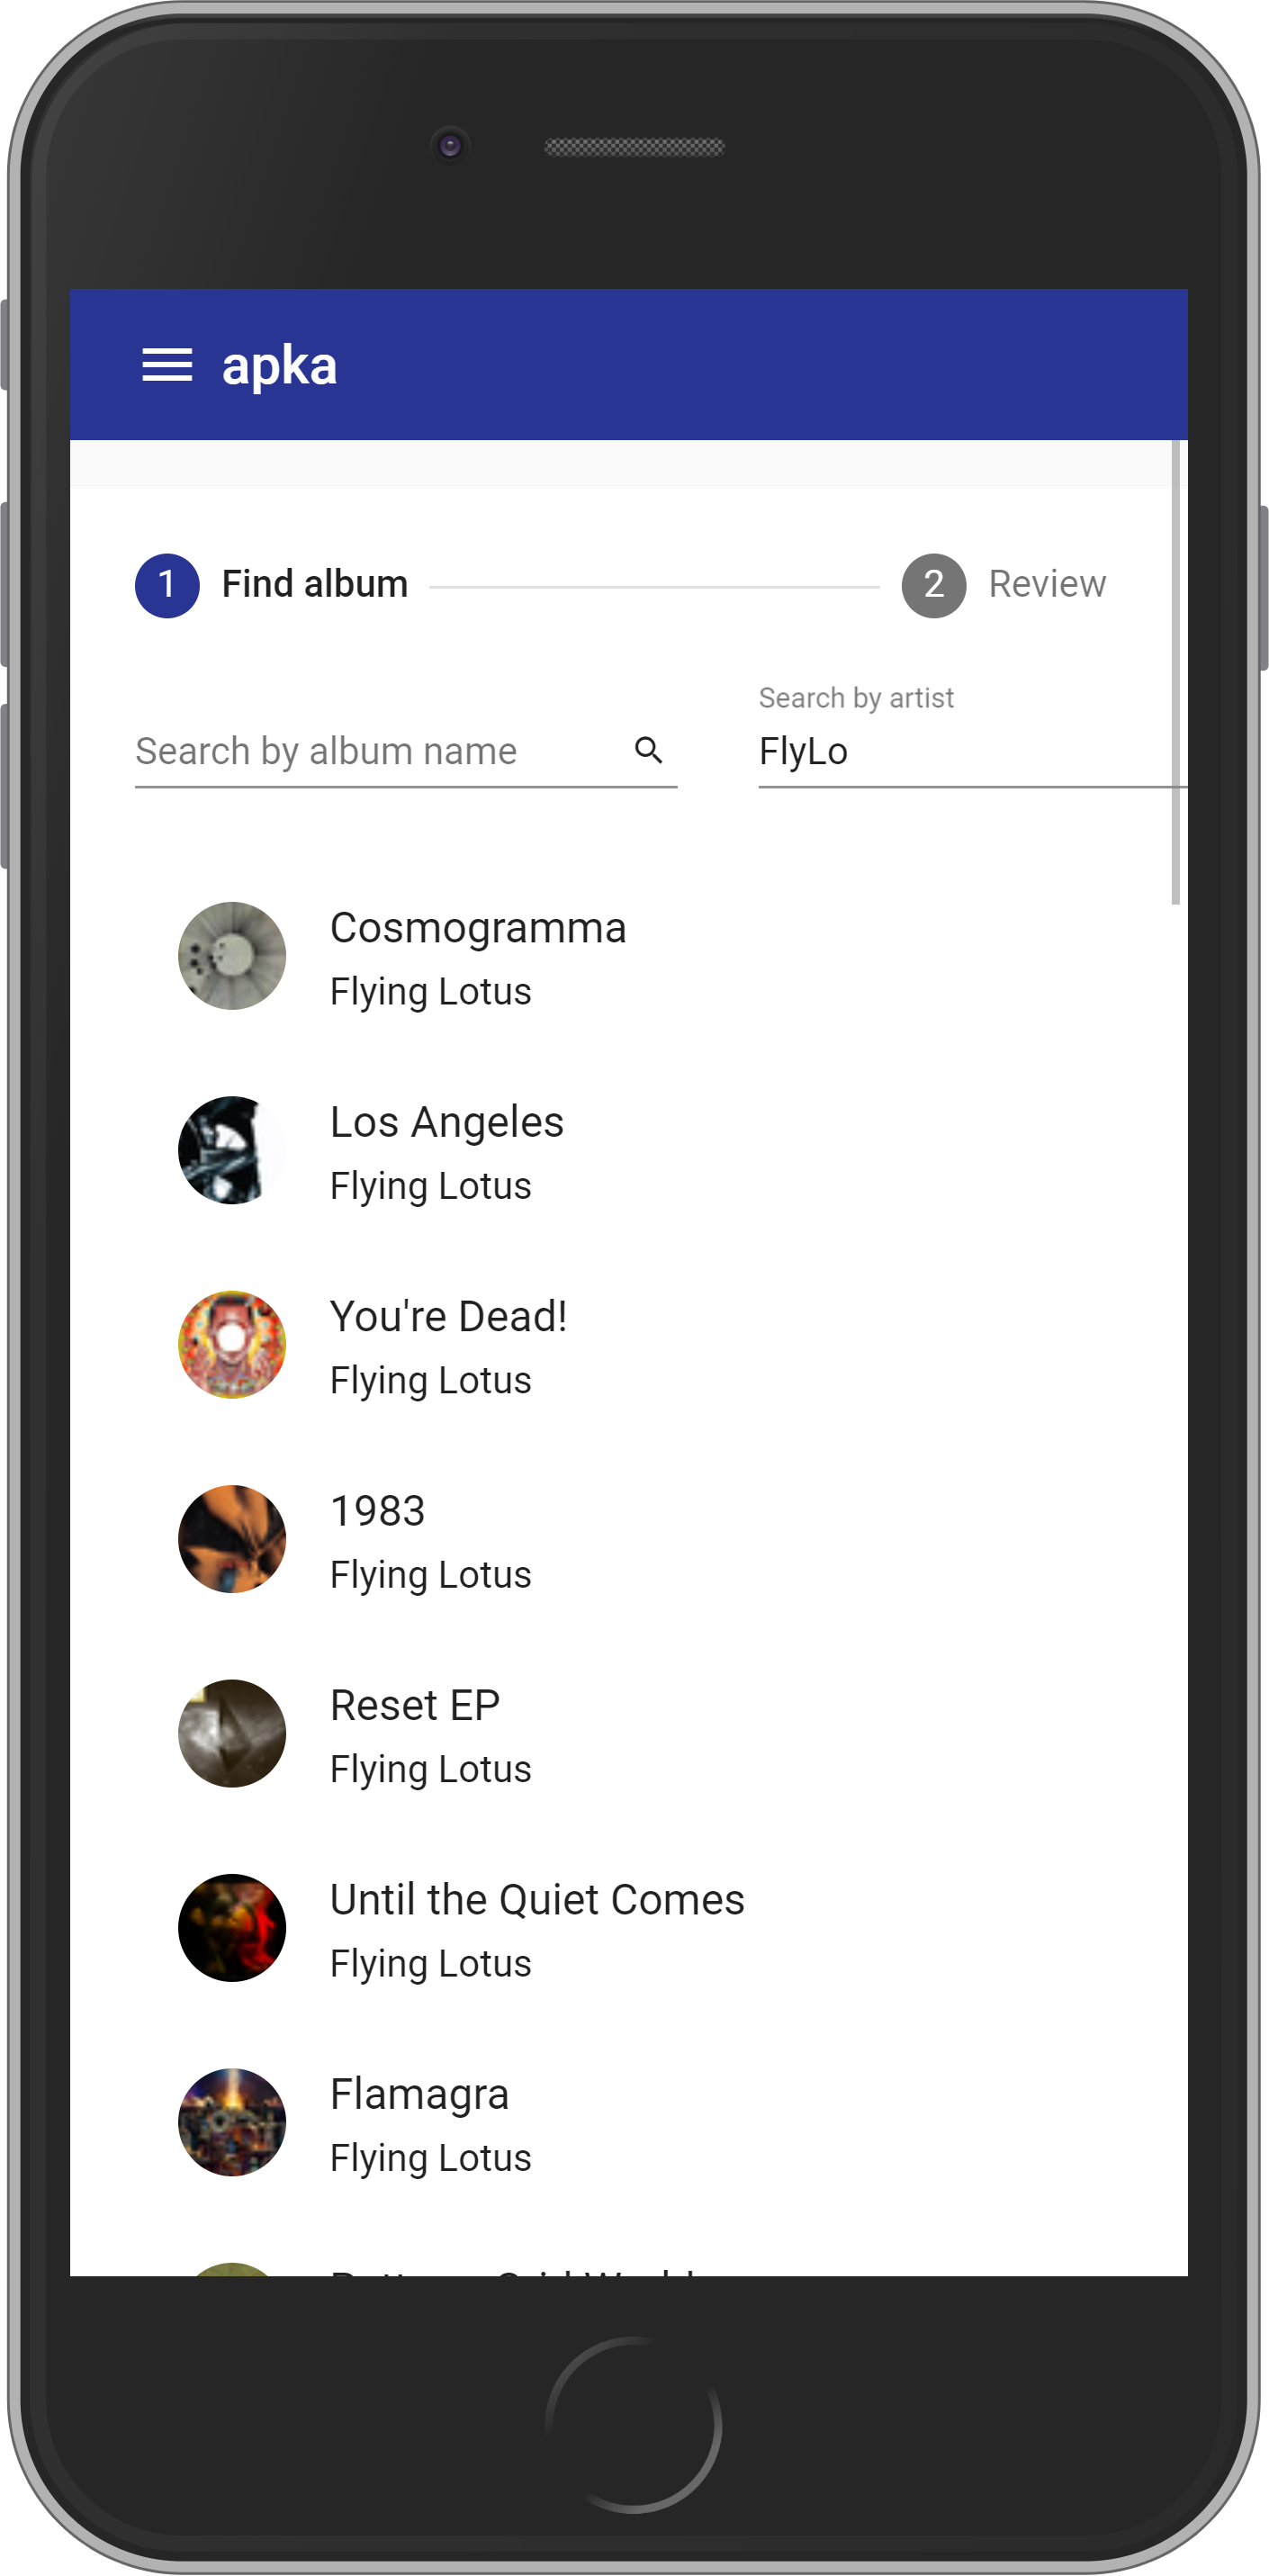
\includegraphics[width=0.9\linewidth]{rys06/search_light.png}
		\end{minipage}%
		\begin{minipage}{0.5\textwidth}
			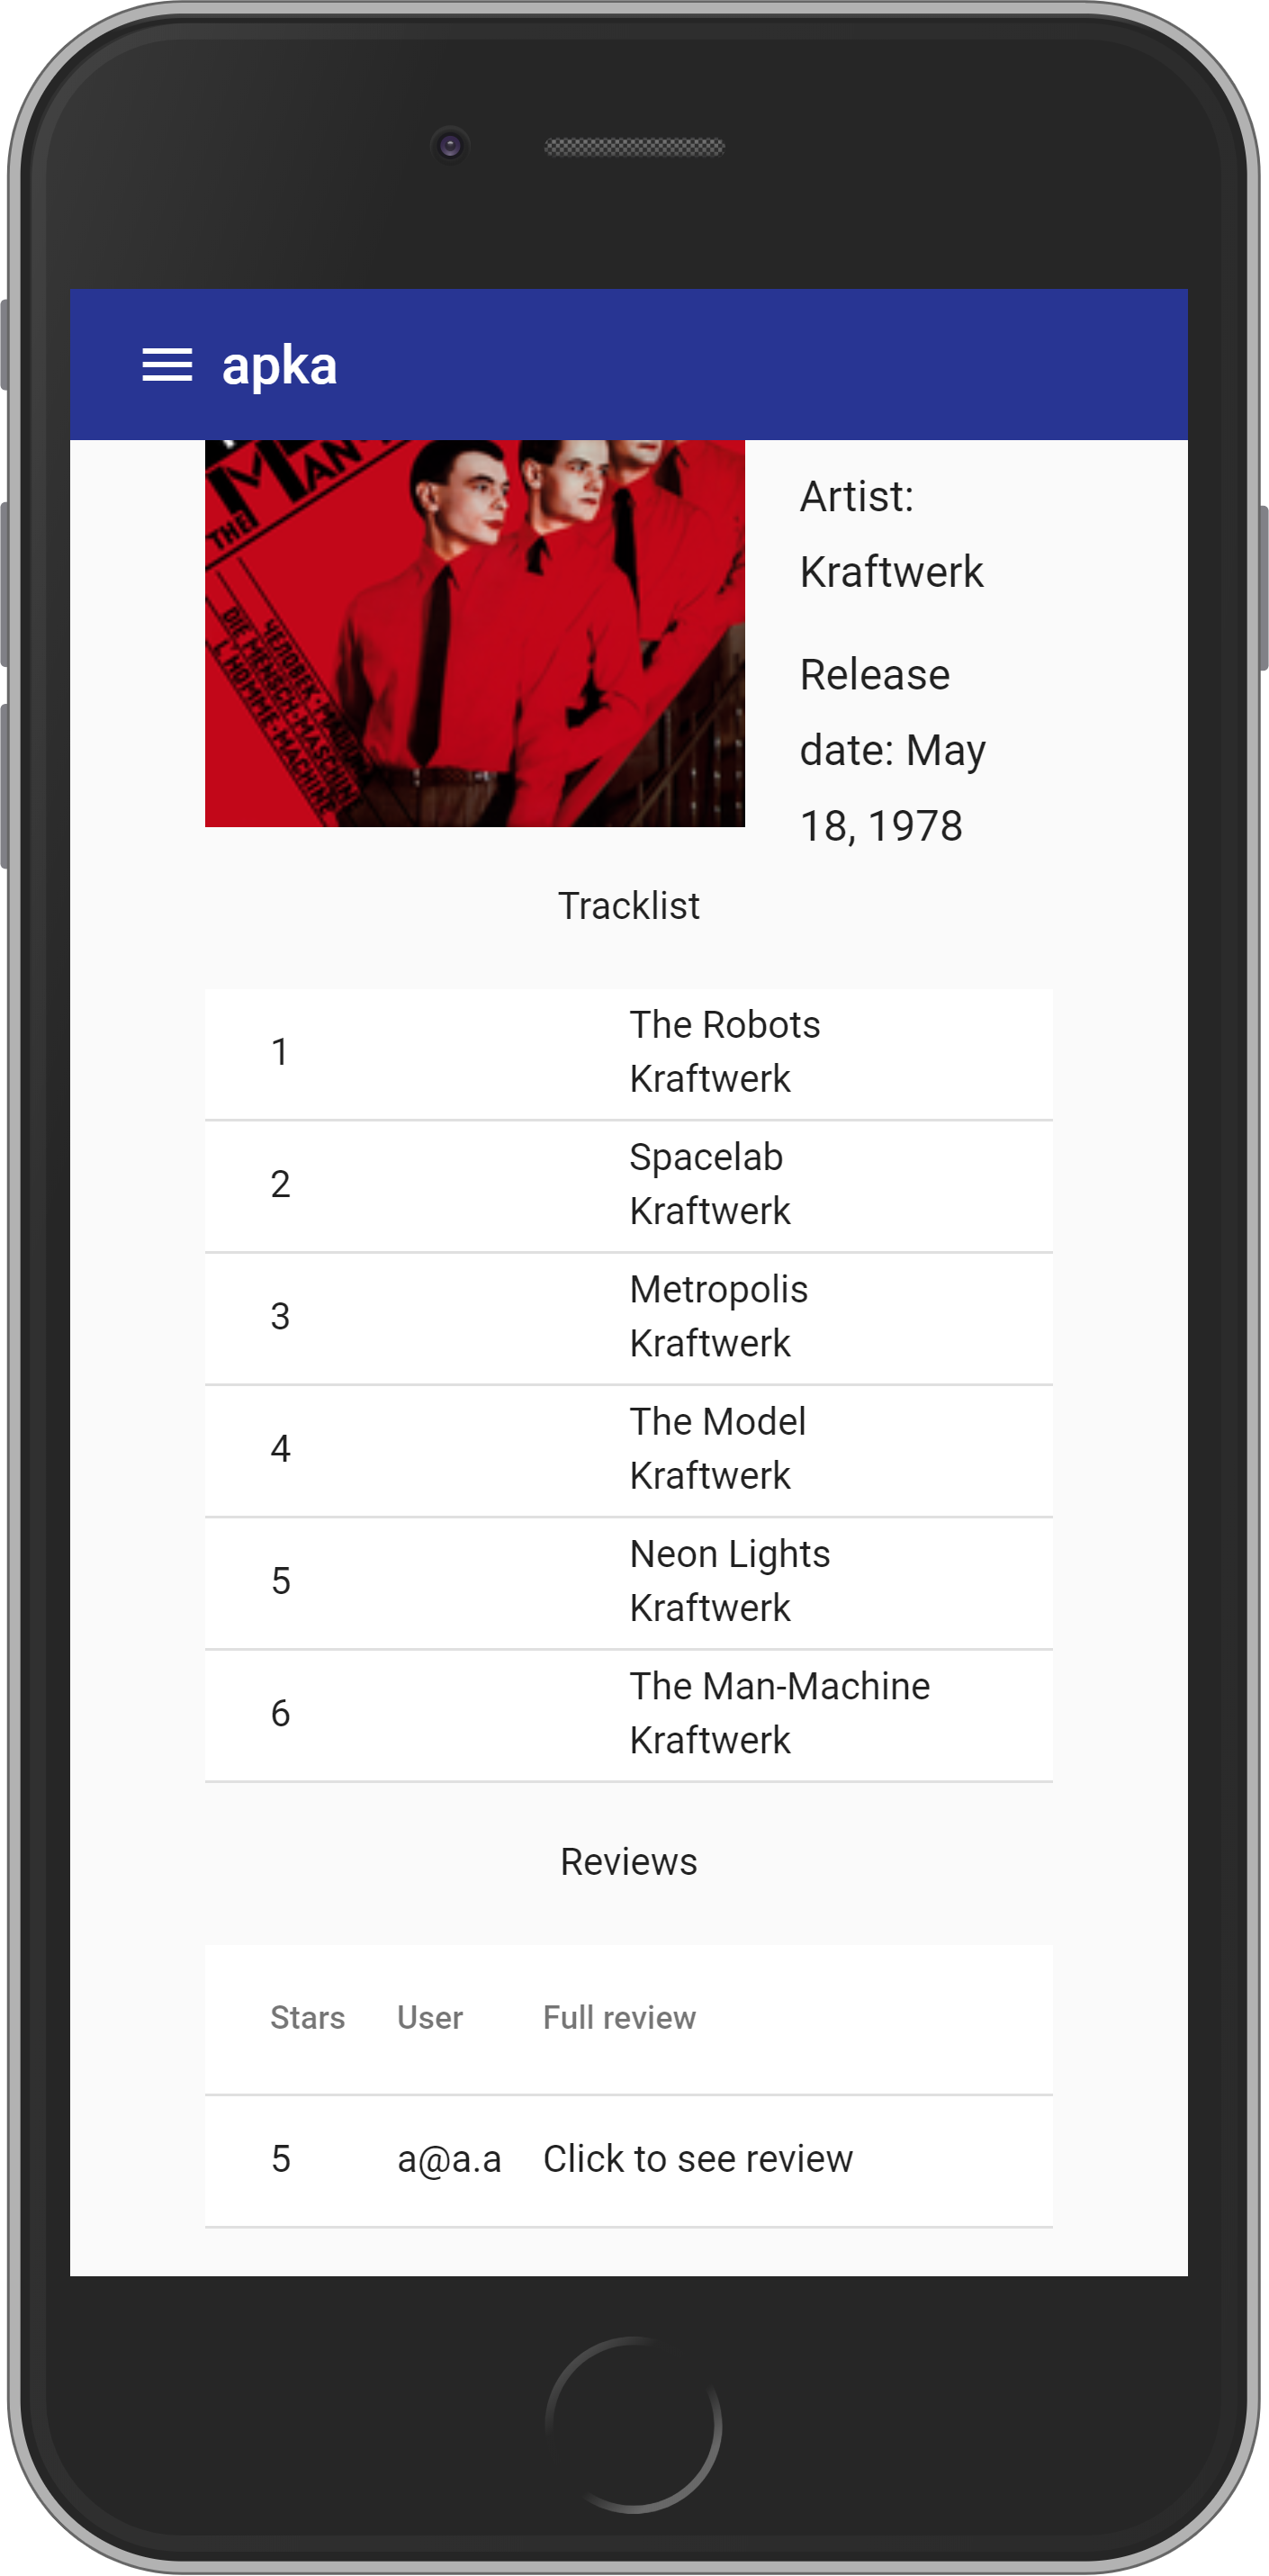
\includegraphics[width=0.9\linewidth]{rys06/album_light.png}
		\end{minipage}
		\caption{Widoki w jasnym motywie}
		\label{fig:light}
	\end{figure}